\documentclass[a4paper]{article}
\usepackage[utf8]{inputenc}

% Fonte sem serifa com suporte a expressões matemáticas
\usepackage[default,osfigures]{opensans}
\usepackage[bitstream-charter]{mathdesign}
\usepackage[T1]{fontenc}

% Pacote que define o layout da lista de exercícios
% Opções:
% professor   Exibe as respostas e as resoluções (PADRÃO)
% mediador    Exibe apenas as resoluções. Deve ser usado para gerar a versão da lista para os moderadores.
% aluno       Exibe apenas as respostas. Deve ser usado para gerar a versão da lista para os alunos.
\usepackage[aluno]{univesp-le}

\usepackage{amsmath}
\usepackage{graphicx}
\usepackage{siunitx}
\sisetup{locale=FR}
\usepackage{paralist}
\usepackage{wasysym}
\usepackage{hyperref}
\usepackage{booktabs}


% Definições personalizadas
\newcommand\myrightarrow{\quad\Rightarrow\quad}

% Define o nome da disciplina, do professor-autor e as aulas às quais a lista de exercício refere-se
\disciplina{Física II} % = \title
\autor{Ivan Ramos Pagnossin}           % = \author
\aulas{1--10}

\hyphenation{Sa-ben-do Ga-ni-me-des trans-la-ção mo-ver}

\begin{document}

% Imprime o nome da disciplina, do professor-autor e as aulas às quais a lista de exercício refere-se
\maketitle
 
% Cada  inicia um novo exercício, independentemente de tratar-se do enunciado, resposta ou resolução.
%-----------------------------------------------------
\begin{exercicio}
  \begin{inlineenum}
  \inlineitem Determine a força gravitacional que atrai um homem de \SI{65}{kg} a uma mulher de \SI{50}{kg} quando eles estão afastados de \SI{0.5}{m} (considere-os como partículas pontuais).
  \inlineitem Qual é a energia potencial gravitacional dessa interação? 
  \end{inlineenum}
\end{exercicio}

\begin{exercicio*}
  Qual é a aceleração de queda livre de um corpo a uma altitude correspondente à órbita de um veículo espacial, a cerca de \SI{400}{km} acima da superfície da Terra?
\end{exercicio*}

\begin{exercicio}
 Determine a velocidade de escape na superfície de Mercúrio, que possui massa de \SI{3.31e23}{kg} e raio de \SI{2440}{km}.
\end{exercicio}

\begin{exercicio}
 Europa é um satélite do planeta Júpiter, cujo raio é \SI{1569}{km} e a aceleração da gravidade, na sua superfície, de \SI{1.39}{m/s^2}.
\begin{enumerate}
\item Calcule a velocidade de escape de Europa.
\item Que altura um objeto alcançaria se fosse lançado para cima com uma velocidade de \SI{1.01}{km/s}?
\item Com que velocidade um objeto atingiria o satélite se ele fosse largado de uma altura de \SI{1000}{km}?
\item Calcule a massa de Europa.
\end{enumerate}
\end{exercicio}

\begin{exercicio}
 Um projétil é lançado em linha reta para cima, a partir da superfície da Terra, com velocidade \SI{15}{km/s}.
Determine a velocidade do projétil quando ele estiver bem afastado da Terra (ignore a resistência do ar. O raio da Terra é \SI{6370}{km}).
\end{exercicio}

\begin{exercicio}
 O asteróide Eros, um dos muitos ``planetas menores'' que orbitam o Sol na região entre Marte e Júpiter, tem raio de \SI{7}{km} e massa \SI{5e15}{kg}.
\begin{enumerate}
\item Se você estivesse em Eros, poderia levantar uma caminhonete de \SI{2000}{kg}?
\item Você poderia correr rápido o suficiente para escapar da atração gravitacional de Eros?\footnote{Nota: os recordes olímpicos de tempo para a corrida de \SI{400}{m} é de \SI{43.49}{s} para homens (Michael Johnson --- EUA, 1996) e de \SI{48.26}{s} para mulheres (Marie-José Pérec --- França, 1996).}
\end{enumerate}
\end{exercicio}

\begin{exercicio}
 Duas partículas puntiformes, cada uma com massa $M$, são fixadas sobre o eixo $y$ em $y=+a$ e $y=-a$.
Determine o campo gravitacional $\vec g$ para todos os pontos sobre o eixo $x$, como função de $x$.
\end{exercicio}

\begin{exercicio}
 Considere um sistema isolado formado por três esferas. Duas delas, de massas $m_1 = \SI{7.16}{kg}$ e $m_2 = \SI{2.53}{kg}$, são separadas por uma distância de centro a centro de \SI{1.56}{m}. A terceira, de massa $m_3 = \SI{212}{g}$, está posicionada a \SI{42}{cm} do centro da esfera $m_2$, ao longo da linha que liga os centros.
\begin{enumerate}
\item Quanto trabalho deve ser realizado por um agente externo para mover a esfera $m_3$ ao longo da linha que liga os centros e posicioná-la a \SI{42}{cm} do centro da esfera $m_1$.
\item Se $m_3$ fosse levado à sua posição final por outro caminho, esse resultado seria diferente? Por quê?
\end{enumerate}
\end{exercicio}

\begin{exercicio}
 Desafio: mostre que a energia total de um objeto em órbita circular é igual à metade de sua energia potencial gravitacional.
Nota: numa órbita circular, a velocidade orbital permanece constante.
\end{exercicio}

\begin{exercicio}
% Leis de Kepler
 O semi-eixo maior da órbita de Júpiter é \SI{5.2}{UA} (unidades astronômicas).\footnote{\SI{1}{UA} = \SI{149 597 871}{km}. Note, entretanto, que você não precisa dessa informação para resolver o exercício.}
Sabendo que o semi-eixo maior da órbita da Terra é \SI{1}{UA}, qual é o período de translação de Júpiter, em anos terrestres?
\end{exercicio}

\begin{exercicio}
 O período de Netuno é de 164,8 anos terrestres. Qual é o valor de sua distância média ao Sol, em unidades astronômicas (UA)?
\end{exercicio}

\begin{exercicio}
 Procure na Internet pelo período $T$ de translação e pelo semi-eixo maior $a$ da órbita de cada planeta do Sistema Solar.\footnote{Ao invés do semi-eixo maior da órbita, você também pode utilizar a distância média entre o planeta e o Sol.}
\begin{enumerate}
\item Faça um gráfico de $T \times a$.

{\footnotesize Dica: utilize UA como unidade de distância e ``anos terrestres'' como unidade de tempo.}

\item Faça um gráfico de $T^2 \times a^3$.

{\footnotesize Dica: ao invés de um gráfico, faça dois: um para os planetas Mercúrio, Vênus, Terra e Marte;
e o outro para Júpiter, Saturno, Urano, Netuno e Plutão.}

\item No gráfico do item anterior, os pontos alinham-se. Qual é o valor do coeficiente angular, no Sistema Internacional de Unidades (SI)?
Compare-o com a constante $4\pi^2/(GM_{\astrosun})$. $G = \SI{6.67e-11}{N.m^2/kg^2}$ é a constante universal da gravidade e $M_{\astrosun} = \SI{1.99e30}{kg}$ é a massa do Sol.
\end{enumerate}
\end{exercicio}

\begin{exercicio}
 A Estação Espacial Internacional move-se segundo uma órbita aproximadamente circular em torno da Terra.
Considerando que ela esteja a \SI{385}{km} acima da superfície da Terra, qual é o período da órbita?
\end{exercicio}

\begin{exercicio*}
 Júpiter é o maior planeta do Sistema Solar. Sua massa é de aproximadamente $M_{\jupiter}=\SI{1.9e27}{kg}$ (318 vezes mais massivo que a Terra) e possui mais de cinquenta luas (satélites naturais) conhecidas. As quatro maiores delas, visíveis da Terra com um pequeno telescópio e descobertas por Galileu Galilei no século XVII, são: Io, Europa, Ganimedes e Calisto. Você, ao reproduzir a observação de Galileu, mediu os seguintes períodos de revolução em torno de Júpiter: \SI{42.5}{h} para Io, \SI{85.2}{h} para Europa, \SI{171.6}{h} para Ganimedes e \SI{400.6}{h} para Calisto.  
Com esses dados \emph{apenas} e conhecendo a constante universal da gravidade, monte o gráfico $T^2 \times a^3$ desse sistema planetário.
\end{exercicio*}

% Use o ambiente respostas para as respostas.
\begin{respostas}
  \begin{exercicio}
    \begin{inlineenum}
      \inlineitem \SI{8.67e-7}{N};
      \inlineitem \SI{-4.33e-7}{J}.
    \end{inlineenum}
  \end{exercicio}
  
  \begin{exercicio*}
    \SI{8.7}{m/s^2}
  \end{exercicio*}
  
  \begin{exercicio}
   \SI{4.25}{km/s}.
  \end{exercicio}
  
  \begin{exercicio}
    \begin{inlineenum}
    \inlineitem \SI{2.09}{km/s};
    \inlineitem \SI{478.9}{km/s};
    \inlineitem \SI{1.303}{km/s};
    \inlineitem \SI{5.13e22}{kg}.
    \end{inlineenum}
  \end{exercicio}

  \begin{exercicio}
   \SI{10}{km/s}.
  \end{exercicio}
  
  \begin{exercicio}
    \begin{inlineenum}
      \inlineitem Sim;
      \inlineitem Não.
    \end{inlineenum}
  \end{exercicio}
  
  \begin{exercicio}
   $\vec g = -\frac{2GMx}{\left(x^2 + a^2\right)^{3/2}}\hat i$
  \end{exercicio}
  
  \begin{exercicio}
    \begin{inlineenum}
      \inlineitem \SI{9.845e-11}{J};
      \inlineitem Não.
    \end{inlineenum}
  \end{exercicio}
  
  \begin{exercicio}
   Dica: a aceleração centrípeta que sustenta a órbita circular é devida à gravidade.
  \end{exercicio}
  
  \begin{exercicio}
   $11,9$ anos terrestres.
  \end{exercicio}
  
  \begin{exercicio}
   \SI{30.1}{UA}.
  \end{exercicio}
  
  \begin{exercicio}
   
  
  \begin{enumerate}
  \item {}\hfill
    \begin{center}
    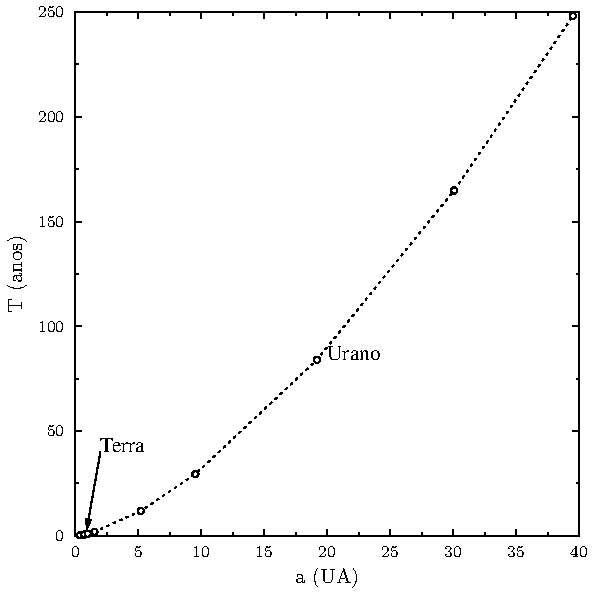
\includegraphics[width=0.45\textwidth]{Txa_planetas_Sistema_Solar}
    \end{center}
    
  \item {}\hfill
  
  \noindent
    \begin{minipage}{0.45\textwidth}
    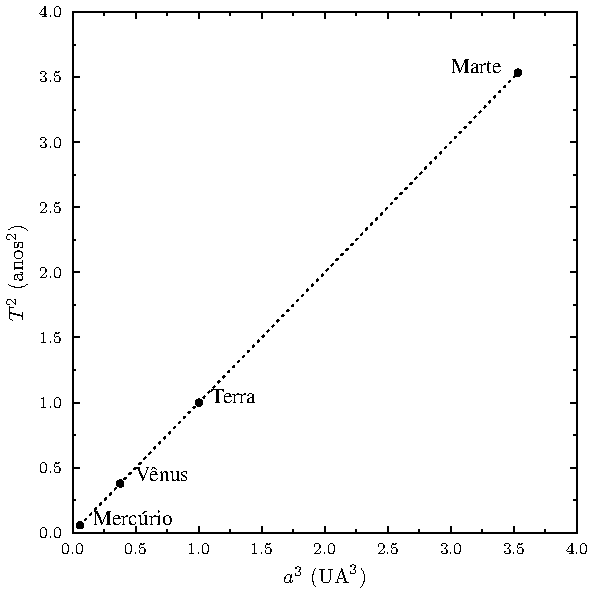
\includegraphics[width=\textwidth]{3a_lei_Kepler_Mercurio-Marte}
    \end{minipage}\hfill
    \begin{minipage}{0.45\textwidth}
    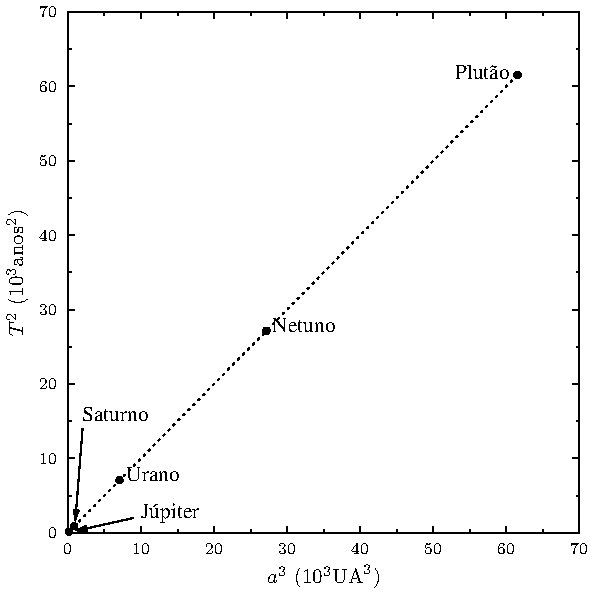
\includegraphics[width=\textwidth]{3a_lei_Kepler_Jupiter-Plutao}
    \end{minipage}
    
  \item O coeficiente angular é igual a $4\pi^2/(GM_{\astrosun}) = \SI{2.97e-19}{s^2/m^3}$.
  
  \end{enumerate}
  \end{exercicio}
  
  \begin{exercicio}
   \SI{92.1}{min}.
  \end{exercicio}
  
  \begin{exercicio*}
    \begin{center}
      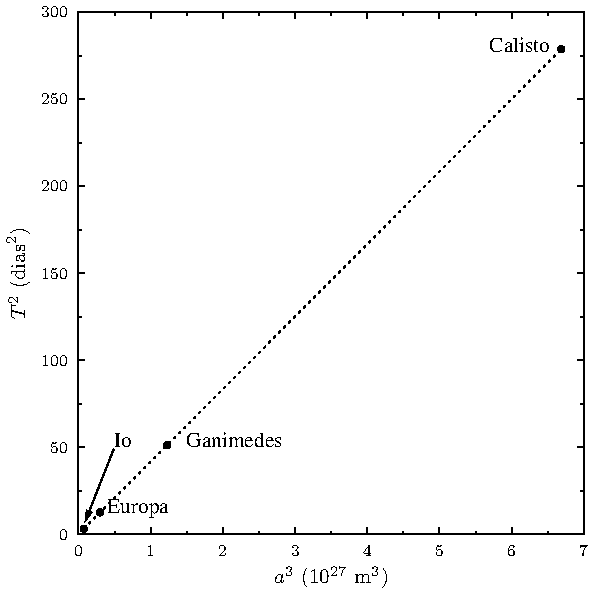
\includegraphics[width=0.5\textwidth]{Io_cia}
    \end{center}
  \end{exercicio*}
\end{respostas}

% Use o ambiente resolucoes para as resoluções.
\begin{resolucoes}

  \begin{exercicio}

  \begin{enumerate}
  
  \item O módulo da força de interação gravitacional entre dois corpos puntiformes é dado pela lei da gravitação universal de Newton:
  \begin{equation*}
  F = \frac{Gm_{\mars}m_{\venus}}{r^2} = \frac{6,67\times10^{-11}\cdot65\cdot50}{(0,5)^2} = \SI{8.67e-7}{\newton}.
  \end{equation*}
  
  \item A energia potencial gravitacional, por outro lado, é igual ao trabalho da força gravitacional, desde a posição $r$ até o infinito.
  Sua expressão é:
  \begin{equation*}
  U_g = -\frac{Gm_{\mars}m_{\venus}}{r} = -\frac{6,67\times10^{-11}\cdot65\cdot50}{0,5} = \SI{-4.33e-7}{\joule}.
  \end{equation*}
  \end{enumerate}
  \end{exercicio}
  
  \begin{exercicio*}
   O módulo da força gravitacional entre um corpo de massa $m$ e a Terra (massa é $M = \SI{5.98e24}{\kilo\gram}$) é dada pela lei da gravitação universal de Newton:
  $F = GmM/r^2$, onde $r$ é a distância entre esse corpo e o centro da Terra.
  Essa força causa uma aceleração em $m$, dada pela segunda lei de Newton: 
  \begin{equation*}
  a = \frac{F}{m} = \frac{GM}{r^2}.
  \end{equation*}
  
  Mas $r = R + h$, onde $R = \SI{6370}{\kilo\metre}$ é o raio da Terra e $h = \SI{400}{\kilo\metre}$, a altitude da órbita.
  Então,
  \begin{equation*}
  a = \frac{GM}{(R + h)^2} = \frac{6,67\times10^{-11}\cdot 5,98\times10^{24}}{\left(6,37\times10^{6}+0,4\times10^{6}\right)^2} = \SI{8.7}{m/s^2},
  \end{equation*}
  que é a aceleração de queda livre (aquela associada à gravidade).
  \end{exercicio*}
  
  \begin{exercicio}
   A velocidade de escape $v_e$ de Mercúrio é, por definição, a velocidade mínima que um corpo deve ter, na superfície, para conseguir livrar-se se sua atração gravitacional.
  ``Livrar-se da sua atração gravitacional'' significa que, no infinito, sua energia cinética terá toda ela sido convertida em energia potencial gravitacional. Ou seja, no infinito temos $K = 0$ (energia cinética nula). Mas no infinito, também a energia potencial gravitacional é nula: 
  \begin{equation*}
  U_g = -\frac{GMm}{r} \myrightarrow \lim_{r \to \infty} U_g = 0.
  \end{equation*}

  Ou seja, a energia mecânica do corpo é nula no infinito: $E = U_g + K = 0$.
  Mas a força gravitacional é conservativa, de modo que $E = 0$ a qualquer distância $r$ do planeta, inclusive na sua superfície, onde $r = R$.
  Nessa posição, a energia mecânica do corpo é:
  \begin{equation*}
  E = -\frac{GMm}{R} + \frac{1}{2}mv_e^2 = 0.
  \end{equation*}
  
  Resolvendo essa igualdade para $v_e$ obtemos a expressão da velocidade de escape de Mercúrio:
  \begin{equation*}
  v_e = \sqrt{\frac{2GM}{R}} = \sqrt{\frac{ 2 \cdot 6,67\times10^{-11} \cdot 3,31\times10^{23} }{2,44 \times10^{6}}} = \SI{4.25}{\kilo\metre\per\second}.
  \end{equation*}
  \end{exercicio}
  
  \begin{exercicio}
  
  \begin{enumerate}
  \item A força gravitacional entre Europa e um corpo de massa $m$ na sobre a sua superfície é dada pela lei da gravitação universal de Newton: $F = GMm/R^2$, onde $R$ é o raio de Europa.
  Pela segunda lei de Newton, essa força causa uma aceleração $g = F/m = GM/R^2$ que, pelo enunciado do exercício, é igual a \SI{1.39}{m/s^2}.
  Por outro lado, a velocidade de escape é dada por $\sqrt{\frac{2GM}{R}}$, que pode então ser reescrita assim:
  \begin{align*}
  v_e &= \sqrt{\frac{2GM}{R}} = \sqrt{2\left(\frac{GM}{R^2}\right)R} = \sqrt{2gR} = \sqrt{2\cdot1,39\cdot 1,569\times10^6}\\
      &= \SI{2.09}{\kilo\metre\per\second}.
  \end{align*}
  
  \item A única força considerada no problema é a gravitacional, entre o objeto e Europa.
  Como essa interação conserva a energia mecânica, podemos determiná-la nos dois pontos de interesse, $A$ e $B$, e usar o princípio da conservação da energia mecânica: $E_A = E_B$.

  A situação $A$ é aquela na qual o objeto está na superfície ($r_A = R$), com velocidade inicial $v_A = \SI{1.01}{\kilo\metre\per\second}$;
  a situação $B$ é aquela na qual toda a energia cinética do objeto foi convertida em energia potencial gravitacional: $r_B = R + h$ e $v_B = 0$.
  $h$ é a altura, acima da superfície de Europa, que o objeto atinge.
  Deste modo, temos:
  \begin{align*}
  E_A &= U_g(r_A) + K(v_A) = -\frac{GMm}{R} + \frac{1}{2}mv_A^2 \\
  E_B &= U_g(r_B) + K(v_B) = -\frac{GMm}{R+h}.
  \end{align*}
  
  Usando $E_A = E_B$ e isolando $h$:
  \begin{gather*}
  E_A = E_B \myrightarrow -\frac{GMm}{R} + \frac{1}{2}mv_A^2 = -\frac{GMm}{R+h} \myrightarrow\\
  \myrightarrow\left(\frac{GM}{R^2}\right)R - \frac{1}{2}v_A^2 = \left(\frac{GM}{R^2}\right)\frac{R^2}{R+h} \myrightarrow\\
  \myrightarrow gR - \frac{1}{2}v_A^2 = g\frac{R^2}{R+h} \myrightarrow h = \frac{gR^2}{gR-v_A^2/2}-R.
  \end{gather*}
  
  Manipulando um pouco mais essa expressão para $h$, obtemos um resultado equivalente, mas que requer menos contas:
  \begin{equation*}
  h = \left(\frac{2g}{v_A^2} - \frac{1}{R}\right)^{-1} = \left[\frac{2\cdot 1,39}{\left(1,01\times10^{3}\right)^2} - \frac{1}{1,569\times10^{6}}\right]^{-1} = \SI{478}{\kilo\metre}.
  \end{equation*}

  \item Conceitualmente, esse problema é análogo ao anterior: a energia mecânica na situação inicial é:
  \begin{equation*}
  E_A = -\frac{GMm}{R+h},
  \end{equation*}
  já que o objeto parte do repouso.
  Durante sua queda livre em direção à superfície do planeta, parte dessa energia potencial gravitacional é convertida em energia cinética.
  Assim ele atinge a superfície com velocidade $v_B$ tal que:
  \begin{equation*}
  E_B = -\frac{GMm}{R} + \frac{1}{2}mv_B^2.
  \end{equation*}
  Como $E_A = E_B$, obtemos daí que:
  \begin{equation*}
  v_B^2 = \frac{2gRh}{R+h} = \frac{2\cdot1,39\cdot1,569\time10^{6}\cdot10^6}{1,569\times10^{6}+10^{6}} \myrightarrow v_B = \SI{1.303}{\kilo\metre\per\second}.
  \end{equation*}

  \item Como $g=GM/R^2$, obtemos imediatamente que:
  \begin{equation*}
  M = \frac{gR^2}{G} = \frac{1,39\cdot \left(1,569\times10^{6}\right)^2}{6,67\times10^{-11}} = \SI{5.13e22}{\kilo\gram}.
  \end{equation*}
  
  \end{enumerate}
  \end{exercicio}
  
  \begin{exercicio}
   Considere as duas situações $A$ e $B$: em $A$ o projétil está na superfície da Terra ($r = R = \SI{6.37e6}{\metre}$) e sua velocidade é $v_A = \SI{1.5e4}{\metre\per\second}$;
  em $B$ o projétil está muito afastado da Terra ($r \to \infty$) e sua velocidade é $v_B$, que queremos descobrir.
  Mas como a única força presente nesse problema é a gravitacional, que é conservativa, a energia mecânica em $A$ e em $B$ deve ser a mesma.
  Ou seja,
  \begin{gather*}
  E_A = E_B \myrightarrow -\frac{GMm}{R} + \frac{1}{2}mv_A^2 = -\lim_{r\to\infty}\frac{GMm}{r} + \frac{1}{2}mv_B \myrightarrow\\
  \myrightarrow -\frac{GM}{R} + \frac{1}{2}v_A^2 = \frac{1}{2}v_B^2 \myrightarrow\\
  \myrightarrow v_B^2 = v_A^2 - 2\frac{GM}{R} = v_A^2 - 2gR \myrightarrow v_B = \SI{10}{\kilo\metre\per\second},
  \end{gather*}
  onde utilizamos $g = GM/R^2 = \SI{9.81}{m/s^2}$, a aceleração da gravidade na superfície da Terra, para simplificar.
  \end{exercicio}
  
  \begin{exercicio}
  
  \begin{enumerate}
  \item A intensidade da força necessária para levantar a caminhonete é igual à força-peso dela, que é dada pela lei da gravitação universal de Newton:
  \begin{equation*}
  F = \frac{GMm}{R^2} = \frac{6,67\times10^{-11}\cdot 5\times10^{15}\cdot 2\times10^{3}}{\left(7\times10^{3}\right)^2} = \SI{13.6}{\newton}.
  \end{equation*}
  
  Na Terra, $F$ equivale à força-peso de um objeto cuja massa é $F/g = \SI{1.39}{\kilo\gram}$, com $g = \SI{9.81}{m/s^2}$.
  Ou seja, em Eros essa caminhonete pesaria tanto quanto um haltere de academia, de modo que você conseguiria levantá-la facilmente!
  
  \item Para desvencilhar-se da atração gravitacional de Eros, você precisaria correr tão ou mais rapidamente que a velocidade de escape dele:
  \begin{equation*}
  v_e = \sqrt{2GM/R} = \sqrt{{2\cdot 6,67\times10^{-11}\cdot 5\times10^{15}}/{7\times10^{3}}} = \SI{9.8}{\metre\per\second}.
  \end{equation*}
  
  O recorde masculino (feminino) dos \SI{400}{\metre} é de \SI{43.49}{\second} (\SI{48.25}{\second}), o que corresponde à velocidade de \SI{9.2}{\metre\per\second} (\SI{8.3}{\metre\per\second}), que é menor que $v_e$.
  Portanto, nem mesmo o mais rápido corredor é capaz de correr rapidamente o suficiente para escapar da atração gravitacional de Eros.

  \end{enumerate}
  \end{exercicio}
  
  \begin{exercicio}
   
  Cada partícula produz um campo gravitacional, $\vec g_1$ e $\vec g_2$, cuja intensidade é:
  \begin{equation*}
  g_1 = g_2 = \frac{GM}{r^2},
  \end{equation*}
  onde $r$ é a distância da partícula até o ponto $P$ onde queremos determinar o campo gravitacional resultante (veja a figura abaixo).
  Pela simetria do problema, vemos que a componente $y$ de $\vec g_1$ contrapõe-se precisamente à de $\vec g_2$.
  Deste modo, a componente $y$ do campo gravitacional resultante é nula.
  Por outro lado, a componente $x$ de $\vec g_1$ e de $\vec g_2$ somam-se e apontam no sentido negativo de $x$ (vetorialmente, representamos por $-\hat i$).
  Assim,
  \begin{equation*}
  \vec g = \vec g_1 + \vec g_2 = -2g_1\cos(\theta)\hat i,
  \end{equation*}
  onde $\theta$ é o ângulo associado ao ponto $P$ (figura).
  Mas pelo triângulo-retângulo $OPM$, $\cos(\theta)=x/r$ e $r = \sqrt{x^2 + a^2}$.
  Então,
  \begin{equation*}
  \vec g = -\frac{2GM}{r^2}\frac{x}{r}\hat i = -\frac{2GMx}{\left(x^2 + a^2\right)^{3/2}} \hat i.
  \end{equation*}

  \begin{center}
  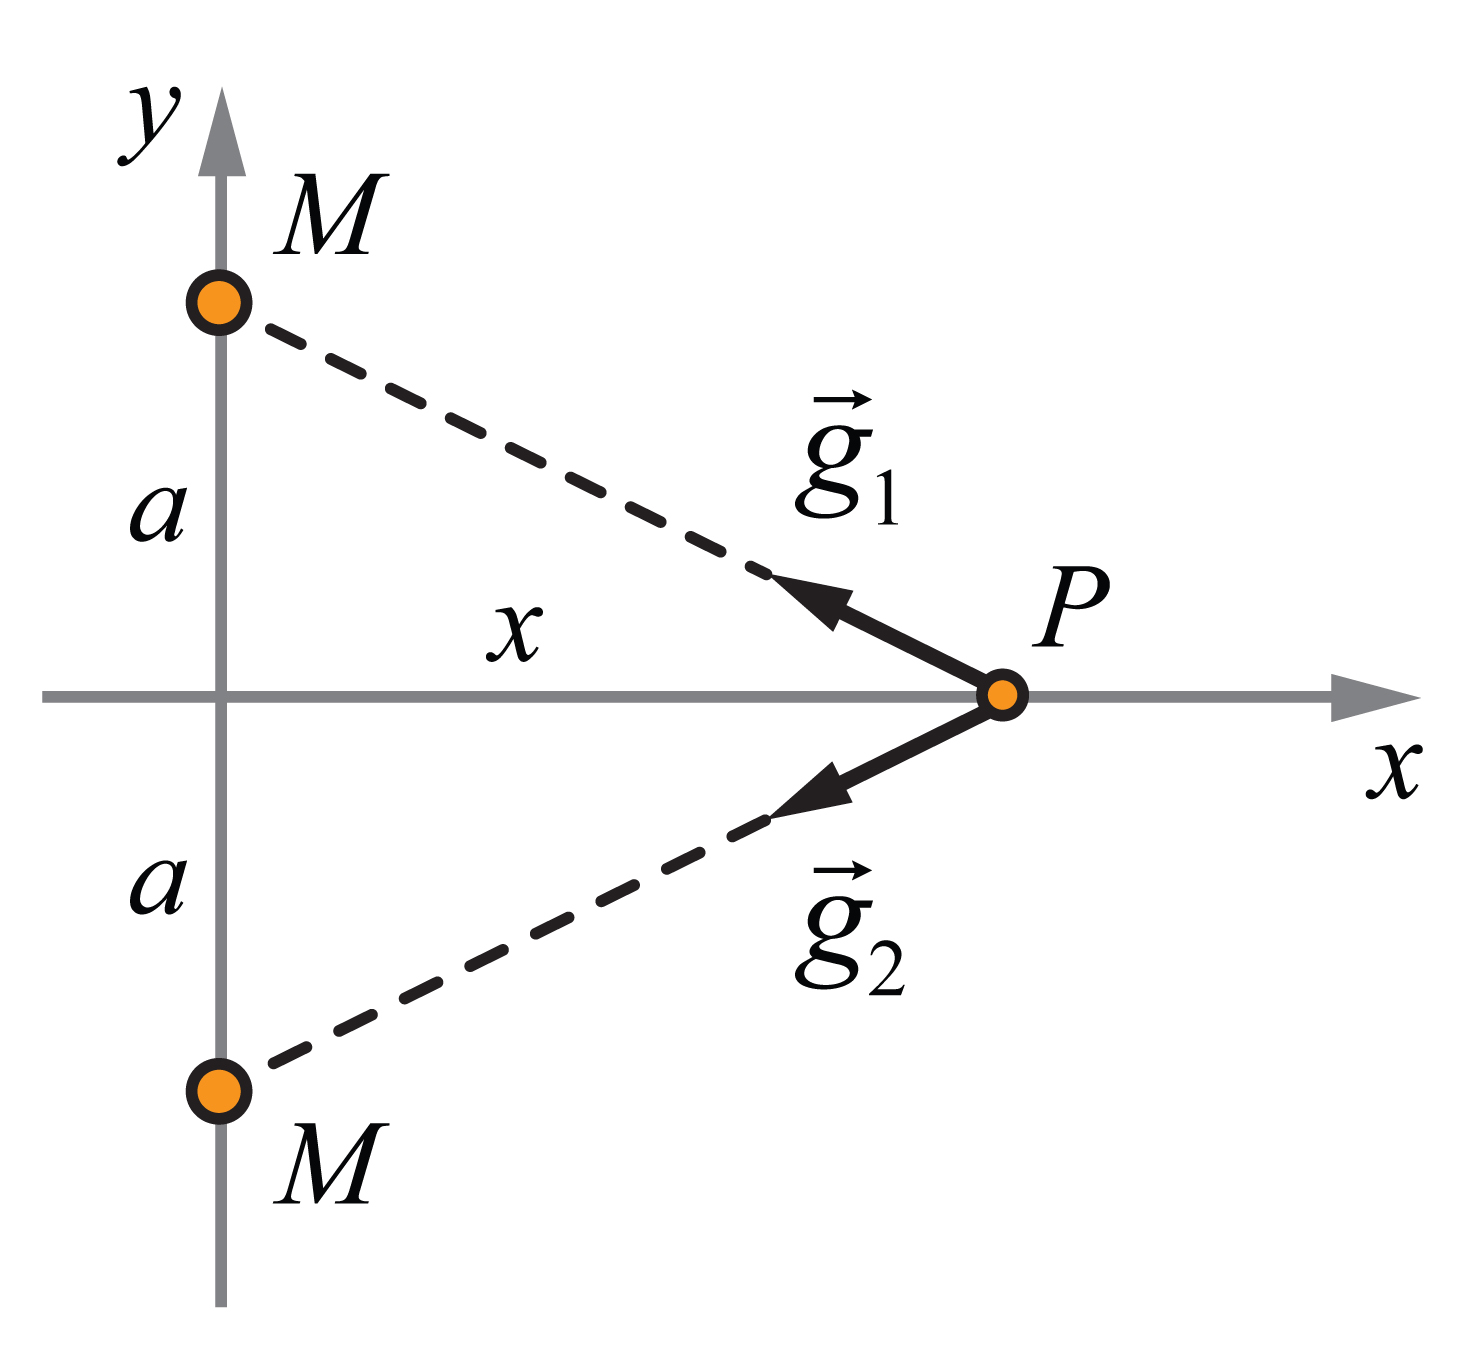
\includegraphics[width=0.45\textwidth]{fig002}
  \end{center}

  Outra forma de resolver esse problema é partir da energia potencial gravitacional: se houvesse um objeto de massa $m$ em $P$, teríamos $U_g = -2GMm/r$, onde $r = \sqrt{x^2 + a^2}$ é a distância entre os corpos $M$ e $m$.
  Como a força gravitacional é derivada da energia potencial gravitacional, temos:
  \begin{equation*}
  \vec F = -\frac{dU}{dx}\hat i = -\frac{d}{dx}\left(-\frac{2GMm}{r}\right)\hat i = -\frac{2GMmx}{\left(x^2 + a^2\right)^{3/2}}\hat i.
  \end{equation*}
  
  Pela segunda lei de Newton, essa força gravitacional causaria em $m$ uma aceleração
  \begin{equation*}
  \vec g = \frac{\vec F}{m} = -\frac{2GMx}{\left(x^2 + a^2\right)^{3/2}}\hat i,
  \end{equation*}
  que é o resultado desejado.  
  \end{exercicio}
  
  \begin{exercicio}
  
  \begin{enumerate}
  \item Considere que $A$ seja a posição inicial e $B$, a final.
  Ao longo do deslocamento entre $A$ e $B$, há duas forças agindo sobre $m_3$: a força gravitacional $F_g(x)$ resultante da interação com $m_1$ e $m_2$ e a força externa $F_e$.
  Deste modo, o trabalho \emph{total} realizado sobre $m_3$ é:
  \begin{align*}
  W_{A\to B} &= \int_{A}^{B}\left(F_g + F_e\right)\, dx = \int_{A}^{B}F_g\, dx + \int_{A}^{B}F_e\, dx \\
             &= W_{A\to B}^{g} + W_{A\to B}^{e},
  \end{align*}
  onde $W_{A\to B}^{g}$ é o trabalho da força gravitacional apenas e $W_{A\to B}^{e}$, da força externa apenas.
  Mas $W_{A\to B} = \Delta K$ (teorema trabalho-energia cinética), onde $\Delta K$ é a variação da energia cinética entre $A$ e $B$.
  Contudo, como a esfera $m_3$ parte do repouso (em $A$) e termina em repouso (em $B$), $\Delta K = 0$.
  Ou seja, o trabalho \emph{total} (ie, das forças gravitacional e externa) deve ser nulo:
  \begin{equation}\label{eq:W}
  W_{A\to B} = W_{A\to B}^{g} + W_{A\to B}^{e} = 0 \myrightarrow W_{A\to B}^{e} = -W_{A\to B}^{g}.
  \end{equation}
  
  Em palavras: o trabalho da força externa, que interessa-nos conhecer, é o oposto do trabalho realizado pela força gravitacional.  
  Resta determinar $W_{A\to B}^{g}$.
  Há duas formas de fazer isso: a primeira delas é calcular diretamente o trabalho da força gravitacional ao longo do deslocamento considerado:
  \begin{equation*}
  W_{A\to B}^{g} = \int_{A}^{B} F_g(x)\,dx.
  \end{equation*}
  
  A outra forma, mais simples, é lembrar que a força gravitacional é conservativa e que, por isso, vale $W_{A\to B}^{g} = -\Delta U_g$.
  Isto é, o trabalho da força gravitacional em levar a esfera $m_3$ de $A$ até $B$ é igual ao oposto da variação da energia potencial gravitacional $U_g$.
  Mas as energias potenciais gravitacional em $A$ e em $B$ são:
  
  \begin{minipage}{0.45\textwidth}
  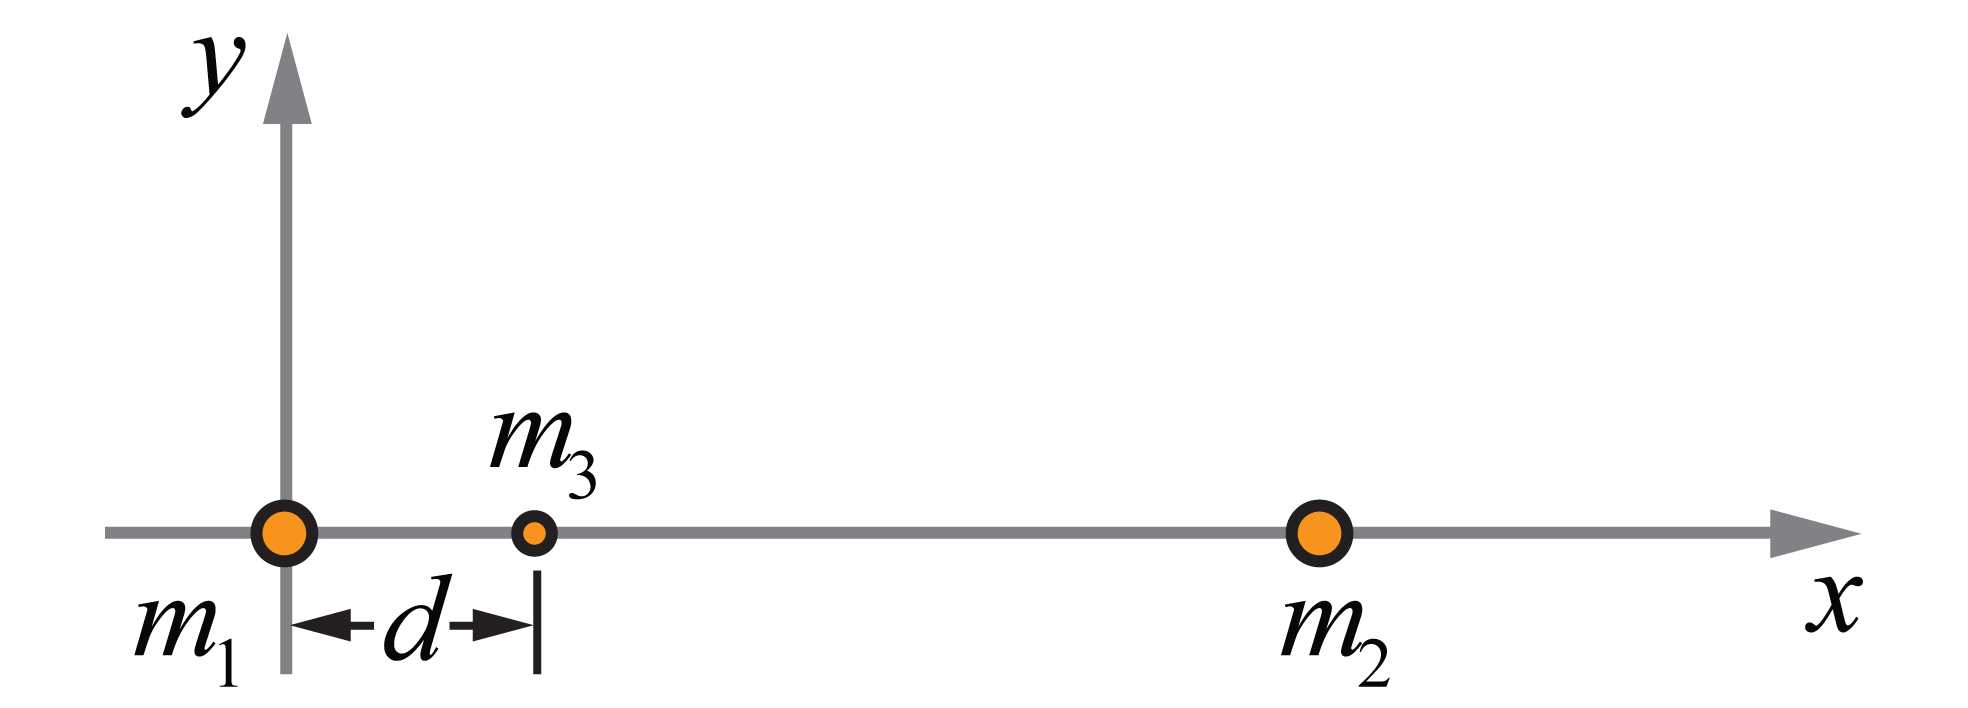
\includegraphics[width=\textwidth]{A}  
  \begin{equation*}
  U_g(A) = -\frac{Gm_1m_3}{d} -\frac{Gm_2m_3}{D-d}
  \end{equation*}
  \end{minipage}\hfill
  \begin{minipage}{0.45\textwidth}
  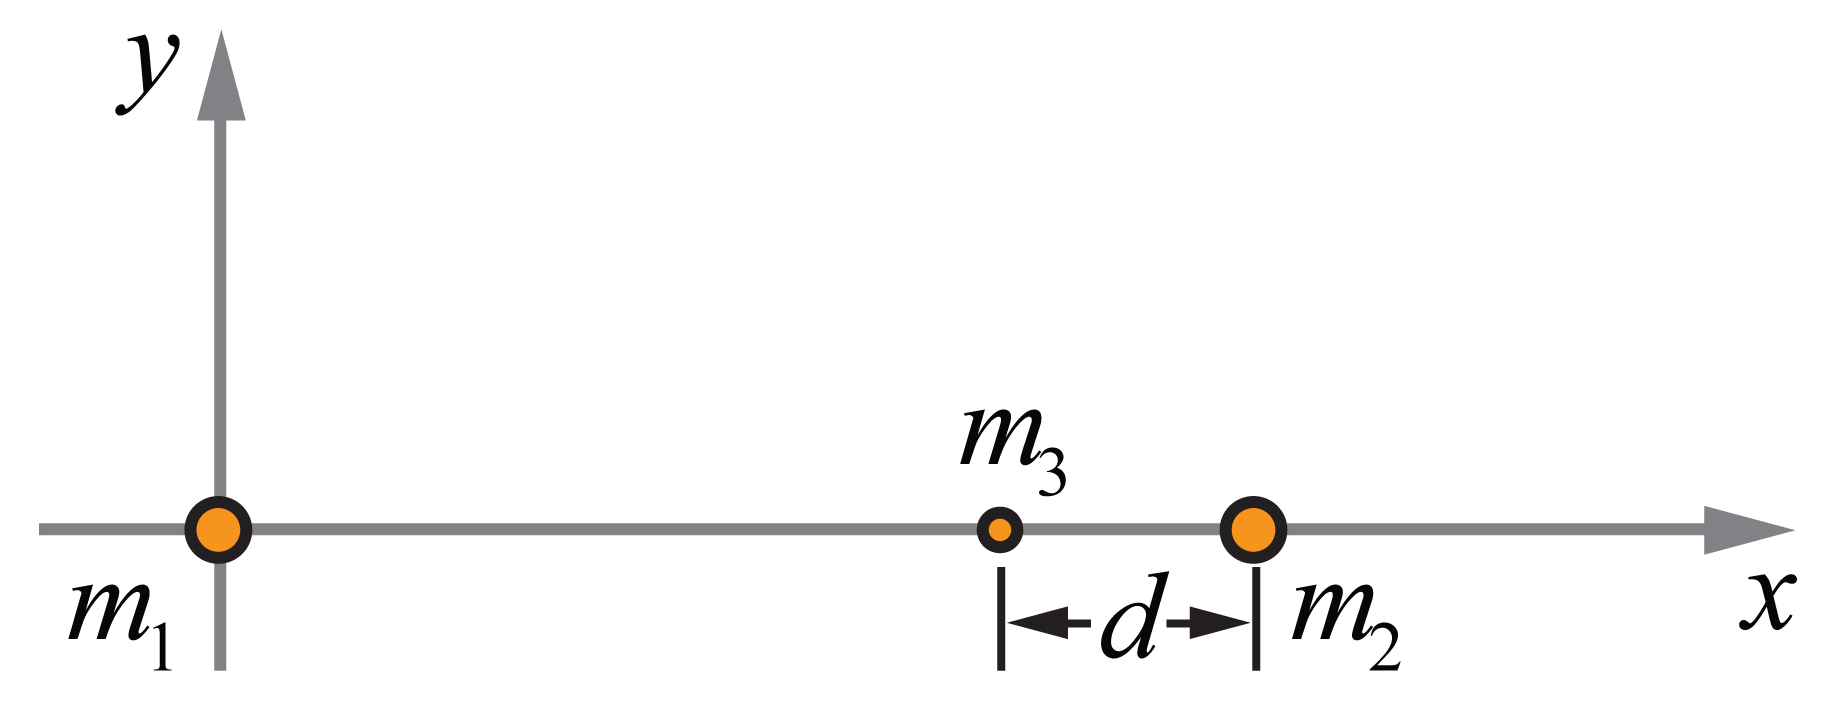
\includegraphics[width=\textwidth]{B}  
  \begin{equation*}
  U_g(B) = -\frac{Gm_1m_3}{D-d} -\frac{Gm_2m_3}{d},
  \end{equation*}
  \end{minipage} 
  
  \medskip
  
  \noindent
  onde $D = \SI{1.56}{\metre}$ é a distância entre as esferas $m_1$ e $m_2$ e $d = \SI{42}{\centi\metre}$.
  Assim,
  \begin{align*}
  W_{A\to B}^{g} &= -\Delta U_g = -\left[U_g(B) - U_g(A)\right]\\
                 &= -\left[\left(-\frac{Gm_1m_3}{D-d} -\frac{Gm_2m_3}{d}\right) -\left(-\frac{Gm_1m_3}{d} -\frac{Gm_2m_3}{D-d}\right)\right]\\
                 &= -Gm_3(m_2-m_1)\left(\frac{1}{D-d}-\frac{1}{d}\right)\\
                 %&= -6,67\times10^{-11}\cdot 0,212 \cdot (2,53-7,16)\cdot \left(\frac{1}{1,56-0,42} - \frac{1}{0,42}\right)\\
                 &= -\SI{9.845e-11}{\joule}.
  \end{align*}

  Finalmente, levando esse resultado em \eqref{eq:W}, obtemos a resposta desejada:
  \begin{equation*}
  W_{A\to B}^{e} = \SI{9.845e-11}{\joule}.
  \end{equation*}
  
  

  \item Como a força gravitacional é conservativa, seu trabalho sobre $m_3$ é independente do percurso.
  De fato, $W_{A\to B}^{g} = U_g(A) - U_g(B)$.
  Como consequência da análise no item anterior, também $W_{A\to B}^{e}$ será independente do percurso.
  \end{enumerate}
  \end{exercicio}

  \begin{exercicio}
   Suponha que a órbita em questão tenha raio $a$.
  Neste caso, a energia potencial gravitacional entre o objeto em órbita, de massa $m$, e o objeto no centro da órbita, de massa $M$, é constante: $U_g = -GMm/a$.  
  Nessa órbita circular, a velocidade orbital $v$ do objeto não muda (isso decorre da conservação do momento angular) e a força centrípeta necessária para sustentar esse movimento é dada pela força gravitacional:
  \begin{gather*}
  F_{\text{centrípeta}} = \frac{mv^2}{a} = \frac{GMm}{a^2} = \left(\frac{GMm}{a}\right)\frac{1}{a} = -\frac{U_g}{a} \myrightarrow\\
  \myrightarrow mv^2= -U_g \myrightarrow 2K = -U_g \myrightarrow K = -U_g/2.
  \end{gather*}
  
  Mas a energia mecânica é $E = U_g + K = U_g - U_g/2 = U_g/2$, como queríamos demonstrar.
  \end{exercicio}
  
  \begin{exercicio}
   Pela terceira lei de Kepler,
  \begin{equation*}
  \frac{T_{\jupiter}^2}{a_{\jupiter}^3} = \frac{T_{\earth}^2}{a_{\earth}^3} \myrightarrow T_{\jupiter} = T_{\earth} \left(\frac{a_{\jupiter}}{a_{\earth}}\right)^{3/2} = 1 \cdot \left(\frac{5,2}{1}\right)^{3/2} \approx \SI{11.9}{anos}.
  \end{equation*}
  
  Na expressão acima, $T$ representa o período, $a$ é o semi-eixo maior e os símbolos $\jupiter$ e $\earth$ representam Júpiter e a Terra, respectivamente.
  \end{exercicio}
  
  \begin{exercicio}
   Pela terceira lei de Kepler,
  \begin{equation*}
  \frac{T_{\neptune}^2}{a_{\neptune}^3} = \frac{T_{\earth}^2}{a_{\earth}^3} \myrightarrow a_{\neptune} = a_{\earth} \left(\frac{T_{\neptune}}{T_{\earth}}\right)^{2/3} = 1 \cdot \left(\frac{164,8}{1}\right)^{2/3} \approx \SI{30.1}{UA}.
  \end{equation*}
  
  Na expressão acima, $T$ representa o período, $a$ é o semi-eixo maior e os símbolos $\neptune$ e $\earth$ representam Netuno e a Terra, respectivamente.
  \end{exercicio}
  
  \begin{exercicio}
  
  \begin{enumerate}
  \item O período e o semi-eixo maior dos planetas do Sistema Solar são:
  
  \noindent
  \begin{minipage}[c]{0.45\textwidth}
    \begin{center}
      \begin{tabular}{lcc}
      \toprule\\
      Planeta & $T$ (anos) & $a$ (UA)\\
      \midrule\\
      Mercúrio & 0.387 &0.241\\
      Vênus & 0.723 & 0.615\\
      Terra & 1 &1\\
      Marte & 1.523 &1.88\\
      Júpiter & 5.203 &11.867\\
      Saturno & 9.539 & 29.461\\
      Urano & 19.185 & 84.03\\
      Netuno & 30.061 & 164.815\\
      Plutão & 39.479 & 248.057\\
      \bottomrule
      \end{tabular}
    \end{center}
  \end{minipage}\hfill
  \begin{minipage}[c]{0.45\textwidth}
    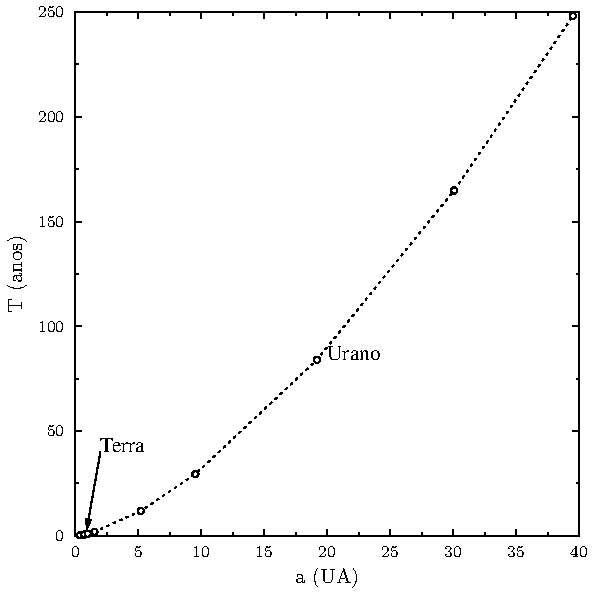
\includegraphics[width=\textwidth]{Txa_planetas_Sistema_Solar}
  \end{minipage}
  
  \noindent
  \textbf{obs.:} há alguns anos, a União Astronômica Internacional criou uma definição formal de planeta, visando classificar diversos outros objetos que orbitam o Sol.
  Como consequência dela, Plutão deixou de ser considerado um planeta. Hoje ele é um ``planeta anão''.
  
  \item O gráfico de $T^2\times a^3$ é mais complicado de fazer, pois a escala varia muito.
  Note, por exemplo, que no gráfico à direita, a abscissa e a ordenada têm um fator mil multiplicando os valores.
  Por isso separamos os planetas em dois grupos: Mercúrio a Marte e Júpiter a Plutão.
  
  \noindent
  \begin{minipage}{0.45\textwidth}
    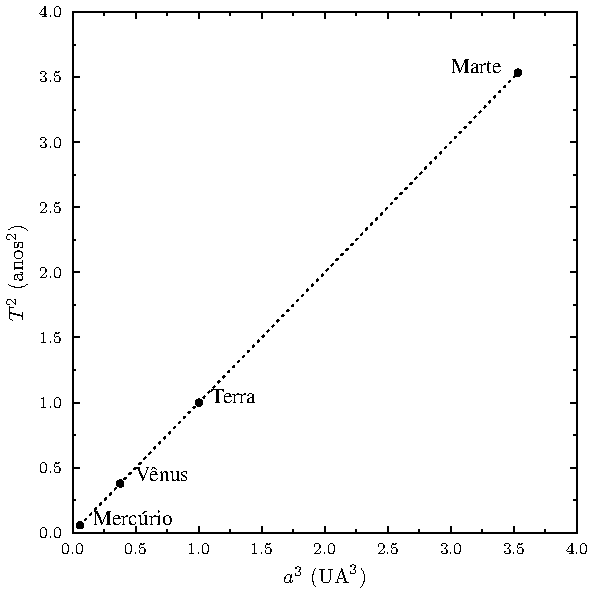
\includegraphics[width=\textwidth]{3a_lei_Kepler_Mercurio-Marte}
  \end{minipage}\hfill
  \begin{minipage}{0.45\textwidth}
    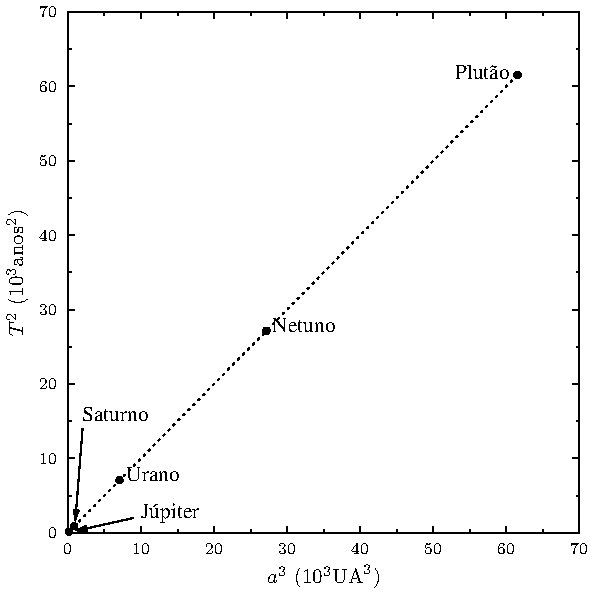
\includegraphics[width=\textwidth]{3a_lei_Kepler_Jupiter-Plutao}
  \end{minipage}\hfill

  \item Tome, por exemplo, o período de translação e o semi-eixo maior da Terra: $T_{\earth} = \SI{3.1536e7}{\second}$ e $a = \SI{1.49597871e11}{\metre}$.
  O coeficiente angular do gráfico $T^2\times a^3$ é:
  \begin{equation*}
  \frac{\left(\SI{3.1536e7}{\second}\right)^2}{\left(\SI{1.49597871e11}{\metre}\right)^3} = 2,97\times10^{-19}.
  \end{equation*}
  
  Esse cálculo pode ser feito para qualquer planeta do Sistema Solar (na verdade, para qualquer astro em órbita do Sol), e o resultado será sempre o mesmo.  
  Por outro lado,
  \begin{equation*}
  \frac{4\pi^2}{M_{\astrosun}G} = \frac{4\pi^2}{1,99\times10^{30}\cdot 6,67\times10^{-11}} = 2,97\times10^{-19}.
  \end{equation*}
  
  Deste modo vemos como Newton conseguiu deduzir, com sucesso, a terceira lei de Kepler (as outras duas também) partindo apenas de sua lei da gravitação universal e das três leis da dinâmica (com isso, Newton demonstrou ainda que as leis que governam o movimento dos astros, na época tidos como domínio do divino, eram as mesmas que valiam na Terra).
  Dito de outra forma, Kepler percebeu que $T^2/a^3$ é o mesmo para todos os planetas do Sistema Solar, mas não sabia explicar o motivo.
  Newton, partindo dos trabalhos de Kepler, compreendeu que esse fator depende exclusivamente da massa do Sol, e deste modo é possível estender a terceira lei de Kepler para qualquer sistema solar ou planetário, como você verá no exercício \ref{ex:Io_cia}.
  
  \end{enumerate}
  \end{exercicio}
  
  \begin{exercicio}
   Segundo a versão de Newton da terceira lei de Kepler, $T^2 = \frac{4\pi^2}{GM_{\earth}}a^3$, onde $T$ é o período da órbita da estação espacial, $M_{\earth}$ é a massa da Terra e $a$ é o semi-eixo maior da órbita da estação espacial.
  Mas $a = R_{\earth} + h$, onde $h$ é a altura da órbita (medida a partir da superfície da Terra e dada no enunciado do exercício).
  Então,
  \begin{equation*}
  T^2 = \frac{4\pi^2}{GM_{\earth}} a^3 = \frac{4\pi^2}{GM_{\earth}} \left(R_{\earth} + h\right)^3 = \frac{4\pi^2}{gR_{\earth}^2} \left(R_{\earth} + h\right)^3,
  \end{equation*}
  onde na última passagem utilizamos $g = GM_{\earth}/R_{\earth}^2$, a aceleração da gravidade na superfície da Terra.
  Agora resta fazer a conta:
  \begin{equation*}
  T = \frac{2\pi}{\sqrt{g}R_{\earth}}\left(R_{\earth}+h\right)^{3/2} = \SI{5529}{s} = \SI{92.1}{min}.
  \end{equation*}
  \end{exercicio}
  
  \begin{exercicio*}
  \label{ex:Io_cia} Para o sistema planetário de Júpiter, vale $T^2 = 4\pi^2 a^3/\left(GM_{\jupiter}\right)$, onde $T$ é o período orbital de qualquer satélite (natural ou artificial) e $a$, seu semi-eixo maior.
  \begin{equation*}
  C = \frac{4\pi^2}{GM} = \frac{4\pi^2}{6,67\times10^{-11}\cdot 1,9\times10^{27}} = 3,11\times10^{-16}.
  \end{equation*}
  
  Agora, tendo $C$ e os períodos das luas de Júpiter, podemos determinar o semi-eixo maior de cada uma:
  \begin{equation*}
  a_{\text{Io}}^3 = \frac{T_{\text{Io}}^2}{C} = \frac{\left(42.5\cdot 60\cdot 60\right)^2}{3,11\times10^{-16}} \myrightarrow a_{\text{Io}} \approx \SI{422000}{km} = \SI{0.422e9}{m}
  \end{equation*}
  
  Fazendo o mesmo para os outros satélites, obtemos:
  
  \begin{center}
    \begin{tabular}{lrr}
    \toprule
    Satélite  & $T$ (dias) & $a$ (\SI{1e9}{m}) \\
    \midrule
    Io        &  1,77      & 0,422 \\
    Europa    &  3,55      & 0,671 \\
    Ganimedes &  7,15      & 1,071 \\
    Calisto   & 16,69      & 1,884 \\
    \bottomrule
    \end{tabular}
  \end{center}
  
  Assim, o gráfico de $T^2\times a^3$ fica assim:

  \begin{center}
  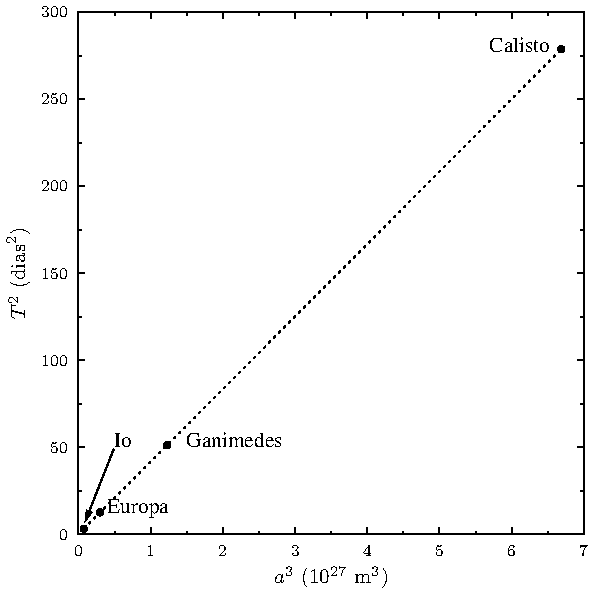
\includegraphics[width=0.5\textwidth]{Io_cia}
  \end{center}
  
  Note que, para melhorar a apresentação do gráfico, o período foi expresso em dias terrestres e o semi-eixo maior, em \SI{1e9}{\metre}.
  \end{exercicio*}
\end{resolucoes}

\end{document}
  